\documentclass{sig-alternate}
%\documentclass[conference]{IEEEtran}
%\documentclass[conference,final]{IEEEtran}

%\usepackage[numbers, sort, compress]{natbib}
\usepackage{graphicx}
\usepackage{amsmath}
\usepackage{amssymb}
\usepackage{color}
\usepackage{ifpdf}
%\usepackage{mdwlist}

%\usepackage{dcolumn}
\usepackage{float}
\usepackage[utf8]{inputenc}
\usepackage{multirow}
\usepackage{rotating}
\usepackage{subfigure}



%\usepackage[numbers, sort, compress]{natbib}
%\usepackage{latex8}
%\usepackage{float}
%\usepackage{times}    
\usepackage{url}
\usepackage{booktabs}
\usepackage{listings}   
\usepackage{paralist}    
\usepackage{wrapfig}    
%\usepackage[footnotesize,it]{caption}
\usepackage{multirow}
\usepackage{ifpdf}
%\usepackage{srcltx}
%\usepackage{subfigure}
\usepackage{xspace}
\usepackage{keyval}  
\usepackage{color}
\usepackage{comment}

\definecolor{listinggray}{gray}{0.95}
\definecolor{darkgray}{gray}{0.7}
\definecolor{commentgreen}{rgb}{0, 0.4, 0}
\definecolor{darkblue}{rgb}{0, 0, 0.4}
\definecolor{middleblue}{rgb}{0, 0, 0.7}
\definecolor{darkred}{rgb}{0.4, 0, 0}
\definecolor{brown}{rgb}{0.5, 0.5, 0}

\usepackage[normalem]{ulem}
\makeatletter
\def\cyanuwave{\bgroup \markoverwith{\lower3.5\p@\hbox{\sixly \textcolor{cyan}{\char58}}}\ULon}
\def\reduwave{\bgroup \markoverwith{\lower3.5\p@\hbox{\sixly \textcolor{red}{\char58}}}\ULon}
\def\blueuwave{\bgroup \markoverwith{\lower3.5\p@\hbox{\sixly \textcolor{blue}{\char58}}}\ULon}
\font\sixly=lasy6 % does not re-load if already loaded, so no memory problem.
\makeatother

\newif\ifdraft
\drafttrue
\ifdraft
\usepackage{xcolor}
\newcommand{\onote}[1]{ {\textcolor{cyan} { (***Ole: #1) }}}
\newcommand{\terminology}[1]{ {\textcolor{red} {(Terminology used: \textbf{#1}) }}}
\newcommand{\owave}[1]{ {\cyanuwave{#1}}}
\newcommand{\jwave}[1]{ {\reduwave{#1}}}
\newcommand{\alwave}[1]{ {\blueuwave{#1}}}
\newcommand{\jhanote}[1]{ {\textcolor{red} { ***shantenu: #1 }}}
\newcommand{\alnote}[1]{ {\textcolor{green} { ***andreL: #1 }}}
\newcommand{\amnote}[1]{ {\textcolor{blue} { ***andreM: #1 }}}
\newcommand{\smnote}[1]{ {\textcolor{brown} { ***sharath: #1 }}}
\newcommand{\pmnote}[1]{ {\textcolor{brown} { ***Pradeep: #1 }}}
\newcommand{\msnote}[1]{ {\textcolor{cyan} { ***mark: #1 }}}
\newcommand{\mrnote}[1]{ {\textcolor{purple} { ***melissa: #1 }}}
\definecolor{orange}{rgb}{1,.5,0}
\newcommand{\aznote}[1]{ {\textcolor{orange} { ***ashley: #1 }}}
\definecolor{dandelion}{cmyk}{0,0.29,0.84,0}
\newcommand{\mtnote}[1]{ {\textcolor{dandelion} { ***matteo: #1 }}}
\newcommand{\note}[1]{ {\textcolor{magenta} { ***Note: #1 }}}
\else
\newcommand{\onote}[1]{}
\newcommand{\terminology}[1]{}
\newcommand{\owave}[1]{#1}
\newcommand{\jwave}[1]{#1}
\newcommand{\alnote}[1]{}
\newcommand{\amnote}[1]{}
\newcommand{\aznote}[1]{}
\newcommand{\athotanote}[1]{}
\newcommand{\smnote}[1]{}
\newcommand{\pmnote}[1]{}
\newcommand{\jhanote}[1]{}
\newcommand{\msnote}[1]{}
\newcommand{\mtnote}[1]{}
\newcommand{\note}[1]{}
\newcommand{\mrnote}[1]{}
\fi

\newcommand{\cloud}{cloud\xspace}
\newcommand{\clouds}{clouds\xspace}
\newcommand{\pilot}{Pilot\xspace}
\newcommand{\pilots}{Pilots\xspace}
\newcommand{\pilotjob}{Pilot-Job\xspace}
\newcommand{\pilotjobs}{Pilot-Jobs\xspace}
\newcommand{\pilotcompute}{Pilot-Compute\xspace}
\newcommand{\pilotcomputes}{Pilot-Computes\xspace}
\newcommand{\pilotdata}{Pilot-Data\xspace}
\newcommand{\pilotdataservice}{Pilot-Data Service\xspace}
\newcommand{\pilotcomputeservice}{Pilot-Compute Service\xspace}
\newcommand{\computedataservice}{Compute-Data Service\xspace}
\newcommand{\pilotmapreduce}{PilotMapReduce\xspace}
\newcommand{\mrmg}{MR-Manager\xspace}
\newcommand{\pstar}{P*\xspace}
\newcommand{\pd}{PD\xspace}
\newcommand{\pj}{PJ\xspace}
\newcommand{\pjs}{PJs\xspace}
\newcommand{\pds}{Pilot Data Service\xspace}
\newcommand{\computeunit}{Compute-Unit\xspace}
\newcommand{\computeunits}{Compute-Units\xspace}
\newcommand{\dataunit}{Data-Unit\xspace}
\newcommand{\dataunits}{Data-Units\xspace}
\newcommand{\du}{DU\xspace}
\newcommand{\dus}{DUs\xspace}
\newcommand{\cu}{CU\xspace}
\newcommand{\cus}{CUs\xspace}
\newcommand{\su}{SU\xspace}
\newcommand{\sus}{SUs\xspace}
\newcommand{\schedulableunit}{Schedulable Unit\xspace}
\newcommand{\schedulableunits}{Schedulable Units\xspace}
\newcommand{\cc}{c\&c\xspace}
\newcommand{\CC}{C\&C\xspace}
\newcommand{\up}{\vspace*{-1em}}
\newcommand{\upp}{\vspace*{-0.5em}}
\newcommand{\numrep}{8 }
\newcommand{\samplenum}{4 }
\newcommand{\tmax}{$T_{max}$ }
\newcommand{\tc}{$T_{C}$ }
\newcommand{\tcnsp}{$T_{C}$}
\newcommand{\bj}{BigJob\xspace}
\newcommand{\MW}{Master-Worker\xspace}
\newcommand{\panda}{PanDA\xspace}
\newcommand{\apples}{AppLeS\xspace}

\newcommand{\I}[1]{\textit{#1}\xspace}
\newcommand{\B}[1]{\textbf{#1}\xspace}
\newcommand{\T}[1]{\texttt{#1}\xspace}
\newcommand{\C}[1]{\textsc{#1}\xspace}

\lstdefinestyle{myListing}{
  frame=single,   
  backgroundcolor=\color{listinggray},  
  %float=t,
  language=C,       
  basicstyle=\ttfamily \footnotesize,
  breakautoindent=true,
  breaklines=true
  tabsize=2,
  captionpos=b,  
  aboveskip=0em,
  belowskip=-2em,
  %numbers=left, 
  %numberstyle=\tiny
}      

\lstdefinestyle{myPythonListing}{
  frame=single,   
  backgroundcolor=\color{listinggray},  
  %float=t,
  language=Python,       
  basicstyle=\ttfamily \footnotesize,
  breakautoindent=true,
  breaklines=true
  tabsize=2,
  captionpos=b,  
  %numbers=left, 
  %numberstyle=\tiny
}



%  \setlength{\parskip}{0.05ex} % 1ex plus 0.5ex minus 0.2ex}
%  \setlength{\parsep}{0pt}
%  %\setlength{\headsep}{0pt}
%  \setlength{\topskip}{0pt}
%  \setlength{\topmargin}{0pt}
%  %\setlength{\topsep}{0pt}
%  \setlength{\partopsep}{0pt}

% This is now the recommended way for checking for PDFLaTeX:


\ifpdf
\DeclareGraphicsExtensions{.pdf, .jpg, .tif}
\else
\DeclareGraphicsExtensions{.eps, .jpg, .ps}
\fi

\tolerance=1000
\hyphenpenalty=10

\usepackage{lscape}

\usepackage{listings}

\lstnewenvironment{code}[1][]%
{
\noindent
%\minipage{0.98 \linewidth} 
\minipage{1.0 \linewidth} 
\vspace{0.5\baselineskip}
\lstset{
    language=Python,
%    numbers=left,
%    numbersep=4pt,
    frame=single,
    captionpos=b,
    stringstyle=\ttfamily,
    basicstyle=\scriptsize\ttfamily,
    showstringspaces=false,#1}
}
{\endminipage}

\begin{document}
\conferenceinfo{HPDC'13}{2013, New York, USA}
% \conferenceinfo{ECMLS'11,} {June 8, 2011, San Jose, California, USA.}
% \CopyrightYear{2011}
% \crdata{978-1-4503-0702-4/11/06}
% \clubpenalty=10000
% \widowpenalty = 10000

\title{A Fresh Perspective on Pilot-Jobs}

% \alignauthor
% Ben Trovato\titlenote{Dr.~Trovato insisted his name be first.}\\
%        \affaddr{Institute for Clarity in Documentation}\\
%        \affaddr{1932 Wallamaloo Lane}\\
%        \affaddr{Wallamaloo, New Zealand}\\
%        \email{trovato@corporation.com}
% % 2nd. author
% \alignauthor
% G.K.M. Tobin\titlenote{The secretary disavows
% any knowledge of this author's actions.}\\
%        \affaddr{Institute for Clarity in Documentation}\\
%        \affaddr{P.O. Box 1212}\\
%        \affaddr{Dublin, Ohio 43017-6221}\\
%        \email{webmaster@marysville-ohio.com}
% % 3rd. author
% \alignauthor Lars Th{\o}rv{\"a}ld\titlenote{This author is the
% one who did all the really hard work.}\\
%        \affaddr{The Th{\o}rv{\"a}ld Group}\\
%        \affaddr{1 Th{\o}rv{\"a}ld Circle}\\
%        \affaddr{Hekla, Iceland}\\
%        \email{larst@affiliation.org}
% \and  % use '\and' if you need 'another row' of author names
% % 4th. author
% \alignauthor Lawrence P. Leipuner\\
%        \affaddr{Brookhaven Laboratories}\\
%        \affaddr{Brookhaven National Lab}\\
%        \affaddr{P.O. Box 5000}\\
%        \email{lleipuner@researchlabs.org}
% % 5th. author
% \alignauthor Sean Fogarty\\
%        \affaddr{NASA Ames Research Center}\\
%        \affaddr{Moffett Field}\\
%        \affaddr{California 94035}\\
%        \email{fogartys@amesres.org}
% % 6th. author
% \alignauthor Charles Palmer\\
%        \affaddr{Palmer Research Laboratories}\\
%        \affaddr{8600 Datapoint Drive}\\
%        \affaddr{San Antonio, Texas 78229}\\
%        \email{cpalmer@prl.com}
% }

\date{}
\maketitle

\begin{abstract} 
  There is no agreed upon definition of \pilotjobs; however a
  functional attribute of \pilotjobs that is generally agreed upon is
  they are tools/services that support multi-level and/or
  application-level scheduling by providing a scheduling overlay on
  top of the system-provided schedulers.  \aznote{Not sure it is good
    to open our abstract stating the confusion/uncertainity inherent
    in defining Pilot-Jobs...  perhaps first state our motivation for
    this work (``aim(ing) to provide appropriate context, insight, and
    analysis of a \pilotjobs, and thereby bring about a hitherto
    missing consilience...'')  and then state that it's somewhat
    controversial?  I see where it could be eye-catching to outright
    state that there IS controversy/uncertainity though, and that we
    are aiming to quash it.  Making this note to try and figure this
    out :)} Nearly everything else is either specific to an
  implementation, open to interpretation or not agreed upon. For
  example, are \pilotjobs part of the application space, or part of
  the services provided by an infrastructure? We will see that
  close-formed answers to questions such as whether \pilotjobs are
  system-level or application-level capabilities are likely to be
  elusive. Hence, this paper does not make an attempt to provide
  close-formed answers, but aims to provide appropriate context,
  insight and analysis of a large number of \pilotjobs, and thereby
  bring about a hitherto missing consilience in the community's
  appreciation of \pilotjobs.  Specifically this paper aims to provide
  a comprehensive survey of \pilotjobs, or more generically of
  \pilotjob like capabilities.  \aznote{Is a ``comprehensive survey''
    still true given last week's discussion of focusing on
    ``landmark'' pilotjobs?}  A primary motivation for this work stems
  from our experience when looking for an interoperable, extensible
  and general-purpose \pilotjobs; in the process, we realized that
  such a capability did not exist. The situation was however even more
  unsatisfactory: in fact there was no agreed upon definition or
  conceptual framework of \pilotjobs.  To substantiate these points of
  view, we begin by sampling (as opposed to a comprehensive survey)
  ~\onote{a few lines above we say that we're doing a comprehensive
    survey!} some existing \pilotjobs and the different aspects of
  these \pilotjobs, such as the applications scenarios that they have
  been used and how they have been used. The limited but sufficient
  sampling highlights the variation, and also provides both a
  motivation and the basis for developing an implementation agnostic
  terminology and vocabulary to understand \pilotjobs; Section \S3
  attempts to survey the landscape/eco-system of \pilotjobs.  With an
  agreed common framework/vocabulary to discuss and describe
  \pilotjobs, we proceed to analyze the most commonly utilized
  \pilotjobs and in the process provide a comprehensive survey of
  \pilotjobs, insight into their implementations, the infrastructure
  that they work on, the applications and application execution modes
  they support, and a frank assessment of their strengths and
  limitations.  An inconvenient but important question -- both
  technically and from a sustainability perspective that must be
  asked: why are there so many similar seeming, but partial and
  slightly differing implementations of \pilotjobs, yet with very
  limited interoperability amongst them?  Examining the reasons for
  this state-of-affairs provides a simple yet illustrative case-study
  to understand the state of the art and science of tools, services
  and middleware development.  Beyond the motivation to understand the
  current landscape of \pilotjobs from both a technical and a
  historical perspective, we believe a survey of \pilotjobs is a
  useful and timely undertaking as it provides interesting insight
  into understanding issues of software sustainability.
  % believe that a survey of \pilotjobs provides and appreciation for
  % the richness of the \pilotjobs landscape.  is
  % not to discuss the \pstar conceptual framework, but That led to
  % the \pstar model.
\end{abstract}

\section{Introduction} 

The seamless uptake of distributed infrastructures by scientific
applications has been limited by the lack of pervasive and
simple-to-use abstractions at multiple levels – at the development,
deployment and execution stages. Of all the abstractions proposed to
support effective distributed resource utilization, a survey of actual
usage suggested that \pilotjobs were arguably one of the most
widely-used distributed computing abstractions – as measured by the
number and types of applications that use them, as well as the number
of production distributed cyberinfrastructures that support them.
\jhanote{Interestingly we find that \pilotjobs have been used even
  before they were named as such!}

\jhanote{Now develop the following paragraph along the lines of: Why
  have \pilotjobs been successful?}

The fundamental reason for the success of the \pilotjob abstraction is
that \pilotjob liberate applications/users from the challenging
requirement of mapping specific tasks onto explicit heterogeneous and
dynamic resource pools.  In other words, at least in part, due to the
decoupling between task/workload specification and task management.
\pilotjobs also thus shields application from having to load-balance
tasks across such resources.  The \pilotjob abstraction is also a
promising route to address specific requirements of distributed
scientific applications, such as coupled-execution and
application-level scheduling~\cite{ko-efficient,DBLP:conf/hpdc/KimHMAJ10}.

%   \onote{I think the most important reasons why Pilot Jobs being so
%     popular (and re-invented over and over again) is that they allow
%     the execution of small (i.e., singe / few-core) tasks efficiently
%     on HPC infrastrucutre by massively reducing queueing time. HPC
%     sites (from schedulers to policies) have always been (and still
%     are) discrimatory against this type of workload in favor of the
%     large, tightly-coupled ones. Pilot-Jobs try to counteract. While
%     this is certainly not the main story that we want to tell, this
%     should IMHO still be mentioned. } \jhanote{This is definitely one
%     of the main reasons, but as Melissa pointed out it during RADICAL
%     call, it is by no means the only reason. Need to get the different
%     reasons down here.. then find a nice balance and description}

\jhanote{Although pilotjobs have solved/addressed many problems, now
    develop the problem with \pilotjobs themselves..}
A variety of PJ frameworks have emerged: Condor-G/
Glide-in~\cite{condor-g}, Swift~\cite{Wilde2011},
DIANE~\cite{Moscicki:908910}, DIRAC~\cite{1742-6596-219-6-062049},
PanDA~\cite{1742-6596-219-6-062041}, ToPoS~\cite{topos},
Nimrod/G~\cite{10.1109/HPC.2000.846563}, Falkon~\cite{1362680} and
MyCluster~\cite{1652061} to name a few. Although they are all, for the
most parts, functionally equivalent -- they support the decoupling of
workload submission from resource assignment -- it is often impossible
to use them interoperably or even just to compare them functionally or
qualitatively.  The situation is reminiscent of the proliferation of
functionally similar yet incompatible workflow systems, where in spite
of significant a posteriori effort on workflow system extensibility
and interoperability (thus providing post-facto justification of its
needs), these objectives remains difficult if not infeasible.

% \subsection{Prior Work}

\section{A Preliminary Survey of Existing Pilot-Jobs Systems}
\label{sec:survey}
% \onote{OLE's SECTION}\jhanote{Ole, several people are already working
%   in this section. You need to coordinate with existing authors here}
% \onote{I'm not sure if I like how we split up between this section and
%   section 'PILOT-JOB SYSTEMS REVISITED'. This will probably lead to a
%   lot of redundancy and a confusing read. Wouldn't it be better to
%   develop the landscape and vocabulary first and then use that to have
%   a comprehensive discussion on Pilot Jobs? }\jhanote{We have had this
%   discussion several times already! This is a limited sampling... in
%   from the perspective of the developers etc.. before we provide a
%   unifying description and then revisit a larger sample of
%   \pilotjobs}

\mrnote{I don't feel like anything in the next three paragraphs should be here or makes sense. I don't know who wrote it, but can someone please justify their text here?}

The aim here is to develop both an understanding of what \pilotjobs
are and a listing of the different \pilotjobs, e.g. Swift, Condor
Glide-in, DIANE, DIRAC.

A specific implementation of the P* model that worked across a variety of middleware and conceptually unified Pilot-Abstractions, led to 
BigJob~\cite{saga_bigjob_condor_cloud} -- a
SAGA-based \pilotjob, which was used to support a range of
applications, ranging from uncoupled ensembles of molecular dynamics
(MD) simulations~\cite{saga_bigjob_condor_cloud}, to Ensemble-Kalman
filter based applications~\cite{gmac09} with global synchronization to
loosely-coupled MD simulations with pair-wise
synchronization~\cite{async_repex11}.  Although BigJob provided the
syntactical uniformity, i.e., a common API and framework for different
grids, our experience led us to understand that different \pilotjobs
had different semantics and capabilities, and made vast if not
inconsistent assumptions of applications/users. This motivated our
efforts in search of a common minimally complete model of \pilotjobs,
and resulted in the \pstar model~\cite{pstar12}. 


There is an axes with a sliding scale of dependence/coupling to
infrastructure.  It is difficult to assign a single point of coupling,
between \pilotjobs and the environment for like most other tools they
are often used in a variety of ways.  We will simply use ``general
purpose'' as a reference to the variety of (i) application types
(static versus dynamic, DAG versus \aznote{DAG vs... ?}) 
(ii) existence/requirement of
special purpose infrastructure (iii) functional extensibility and/or
modularity and/or coupling to environment.

\subsection{A Functional Approach to Pilot-Jobs}

As the uptake of grids grew, the need for job submission management
via batch queuing systems and middleware access also grew. Many
machines implemented their own batch queuing systems, and oftentimes
these systems varied from machine to machine. Many scientific
communities began running into the same problems: (i) heterogenous
resources, (ii) workload management, and (iii) support of various
applications. There was a need to be able to
harness the power of these heterogeneous resources to run
jobs. \pilotjobs have historically been used as a means of solving
this problem. We briefly discuss some of the specific uses of pilot 
jobs below.

\pilotjobs are most commonly used for the execution of many tasks
through the use of a container job. They are often measured by
their throughput, that is, the number of tasks that they can complete
per second (tps). As such, \pilotjobs are used to achieve
high-throughput, for example, when using genome sequencing techniques
or ensemble-based applications. \pilotjobs have also been used for
parameter sweeps, chained tasks, and loosely-coupled but distinct
tasks. %note to self: cite these with papers

Multi-scale simulations have also benefited from the use of
\pilotjobs. A \pilotjob load balancing algorithm was proposed for
coupled Multi-Physics MPI Simulations \cite{ko-efficient} in which
more processors were assigned to jobs with longer runtimes, so as to
make the simulation take the same amount of wall-clock time between
points when they need to communicate with one another (via MPI).

Some simulations require varying number of tasks to complete -- that
is, 10 tasks may start a program but the results of these tasks may
spawn more tasks to complete. \pilotjobs can be utilized for these
types of dynamic simulations, because once they are active, the agents
have an available slot for executing tasks on a given number of
cores. As more tasks are added to the system, the \pilot can continue
to execute new tasks until the job is considered
complete. Without \pilotjobs, these simulations would have to be
resubmitted to the job queue and wait for their time to become active again~\cite{luckow2009adaptive}. 

\pilotjobs have also been used to avoid queue wait times for many jobs
as well as harness and utilize different resources (with different
batch queueing systems) to do \textit{scale-across} simulations.
As a fault tolerant mechanism, many \pilotjob systems monitor
failed jobs and have the ability to restart them within the given 
time frame of the \pilotjob's total runtime~\cite{1742-6596-219-6-062049,condor-g,nilsson2011atlas}. 

\subsection{Historical Context}
\subsubsection*{The Evolution of \pilotjobs}

In order to appreciate \pilotjobs, we outline the evolution of
\pilot-like capabilities ultimately leading to the creation of an actual
\pilotjob. We present a brief chronological order of \pilotjob-like
systems, beginning with simple Master-Worker applications through
advanced workload management systems.
\\ \\
\noindent \textbf{Pre-\pilotjob Systems:}

The Master-Worker application was adapted to grids as a means of farming tasks from a master to a various number of workers, and could easily be adapted to run in a platform-independent way across the potentially heterogeneous resources~\cite{masterworker, Goux00anenabling}. In the grid computing context, Master-Worker schemes could respond to the dynamically changing resources by adapting the number of workers to match the resource availability. Although Master-Worker schemes were important, they required application modification.

Another application that pre-dates pilot jobs is the BOINC middleware system~\cite{Anderson:2004:BSP:1032646.1033223}. BOINC plays a significant role in distributed computing acting as a Client/Server-based platform which utilizes unused computer cycles on the client-side in order to execute tasks given from the server-side. Applications can be built on top of BOINC for their own scientific endeavors; it was originally built for the SETI@Home project, which uses Internet-connected computers to download and analyze radio telescope data. Most often, these computers are based around the world -- users merely have to download the client program, and it runs in the background on their computer. The data is then aggregated back on the server-side and analyzed. The idea of farming out tasks in a distributed environment including personal computers was the first wide-use of the Client/Server model that essentially made a grid out of many less powerful machines.

As the resources in the grid adopted more and more batch queuing systems, users were forced to submit their jobs individually to a scheduler. Oftentimes, the type of scheduler on a certain machine was different than that of another machine. There was a need for managing the heterogenous, dynamic grid environments, especially in terms of dynamic scheduling. This drove the creation of AppLeS~\cite{Berman:2003:ACG:766629.766632}, a framework for 
application-level scheduling. For this purpose, AppLeS provides an agent that 
can be embedded into an application enabling the application to acquire 
resources (e.\,g.\ via Globus, SSH or Legion) and efficiently schedule tasks 
onto these. Further, AppLeS provides different application templates,
e.\,g.\ for parameter sweep, master-worker and moldable parallel applications.

The rise of application-level scheduling, as in AppLeS, opened new possibilities to Grid environments. The concept of application-level scheduling was extended to include long-term performance prediction in heterogenous Grid environments via the Grid Harvest Service (GHS) system~\cite{ghs}. GHS provides a prediction model that was derived by probability analysis and simulation and useful for large-scale applications in shared environments. Its prediction models and task scheduling algorithms are utilized in the placement of tasks across Grid resources. GHS supports three classes of task scheduling: (i) single task, (ii) parallel processing, and (iii) meta-task. The performance evaluation and modeling in conjunction with task-specific management (such as placement, scheduling, and execution) allows the utilization of many heterogenous resources in an efficient manner.

Although pre-pilot systems, such as AppLeS, gave user-level control of scheduling, queue reservation time still was an issue. This brought about the idea of placeholder scheduling~\cite{Pinchak02practicalheterogeneous, Singh:2008:WTC:1341811.1341822}. A placeholder was a \pilot-like mechanism in that it was an abstraction layer above the various batch queuing systems available on different resources. It held a \textit{place} in the regular batch queue, and when it became active, it could pull tasks to execute. Placeholder scheduling was advantageous in that it did not require any special superuser privileges on the machines, which was something most grid users did not have access to. It also provided a means of load balancing across the different resources. As placeholder scheduling evolved, it came to include dynamic monitoring and throttling of the different placeholders based on the queue times on the machines.

Second generation systems, which will be talked about in depth in Section \ref{sec:pj} encompass complex workload management systems based on \pilots. The idea of a placeholder scheduling proved to be an efficient model for waiting in the resource batch queue only once, but executing many tasks once the placeholder job became available via a pull model. As applications began to utilize distributed cyberinfrastructure, the workloads grew from small sets of short running jobs to many jobs with either short or potentially long runtimes. There was a need for more complex management of these workloads and additional capabilities for user-level control of the tasks that would be executed within the placeholder job. This drove the creation of the modern idea of \pilots. 
 
% Cite: Work Queue: http://www3.nd.edu/~ccl/research/papers/wq-python-pyhpc2011.pdf 
% Work queue is not based on pilots but is an interesting read for ensemble-based scientific applications on grids using python


%For:
%\begin{itemize}
%\item High-Throughput Simulations
%\item Dynamic Simulations
%\item Other - Multi-scale simulations \mrnote{Dynamic load balancing for MPI jobs} 
%\item Avoiding Queue wait times for many jobs
%\item Harness and utilize different resources (with different batch queuing systems) to do runs across all of them
%\end{itemize}

\subsection{Informal Description of Pilot-Job Systems}
\label{sec:pj}
\alnote{AL/MS}

\note{talk about tool development, unregulated cottage industry - Why
  is that? diverse low-level infrastructure, no incentive to use
  multiple infrastructures? External vs.  internal perspective?}

As stated above, \pilotjobs provide the ability to 
distribute workload across multiple systems and
provide an easy way to schedule many jobs at one time. This in turn
improves the utilization of resources, reduces the net wait time of a
collection of tasks, and also prevents saturation of resource batch
queuing systems from high-throughput simulations where many jobs
need to be run at one time.

\subsubsection*{Criteria and Classifications}
\alnote{refine structure: function/non-functional, internal/external}
We assess the \pilotjob-Systems according to the following criteria:
\begin{itemize}
	\item What use cases? What applications types are supported? MPI, ensembles, workflows? Single vs. multi-purpose?
	\item What low-level infrastructures/middleware are supported? How interoperable is the framework (vertically, horizontally)?
	\item Scale of distribution
	\item Internal Architecture (communication \& coordination, central vs. decentral architectures; push vs. pull model, agent-based; number of supported pilots/resources; vertical/horizontal integration...)
	\item Deployment Model: service versus tool/library, application vs. system-level
    \item Abstraction/Programming Model: CLI, Scripting (SWIFT), API, Web service
	\item Performance and Scalability (Task Throughput)
	\item Fault Tolerance
	\item Integration with higher-level tools (e.g. workflow systems, data analysis systems)
	\item Scheduling: supported algorithms, support for application-level 
	scheduling, data-compute scheduling, resource acquisition/release policies, dispatch policies, number of scheduling levels
	\item Support for Data
	\item Security (Single vs. Multi-User)
	\item Deployment Model: centrally hosted vs. application-level library
\end{itemize}

As shown Figure~\ref{fig:figures_classification}, PJ systems operate on
different levels of the distributed computing stack: (i) PJ systems that
solely provide a simple \pilot capability, (ii) systems that provide resource
management capabilities based on \pilots and (iii) applications, tools and
services that utilize \pilots. Higher-level applications and tools either 
provide a highly-integrated vertical framework, which deeply integrates the PJ 
system (e.\,g.\ Swift/Coaster), or rely on a third-party 
\pilotjob framework, e.\,g.\ Pegasus which re-uses on Condor-G for piloting.

\begin{figure}[t]
	\centering
		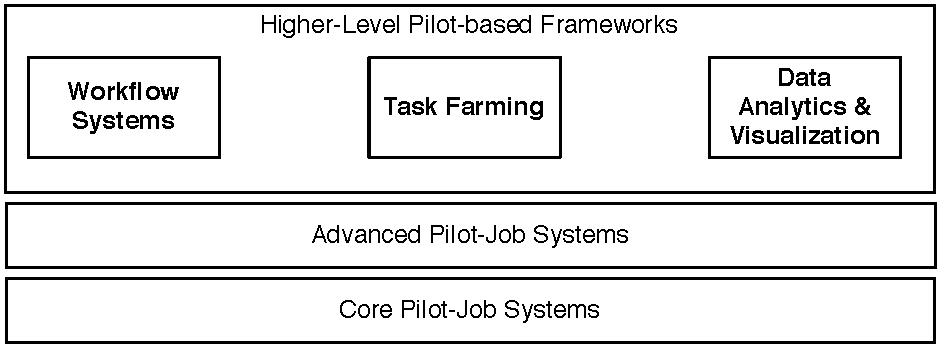
\includegraphics[width=0.45\textwidth]{figures/classification}
	\caption{Pilot-Job Classification: Different PJ systems focus
          on different parts of the distributed computing stack: (i)
          PJ systems that solely provide the \pilot capability, (ii)
          systems that offer resource management capabilities based on
          \pilots and (iii) applications, tools and services that
          utilize \pilots for resource management. \jhanote{we should
            change the ``higher-level pilot-based frameworks'' to
            ``higher-level frameworks that can use pilot-jobs''.}}
        \alnote{mention that these layers are not cleanly separated:
          Pegasus is constraint to a single PJ system (Corral)}
	\label{fig:figures_classification}
\end{figure}


\subsubsection*{Pilot-Job Systems Overview}

\alnote{add pre-pilot; introduce categories before going into details.}

\alnote{fix numbering}

PJ to survey (pilots can fall potentially in on or more categories):
\begin{itemize}
	\item Basic Pilot-Job Systems: \mtnote{I think I understand what simple means here but I think we need to find a better term. See also Ole's comment on using core instead of simple.}
	\begin{itemize}
		\item Condor-G/Glide-In
		\item MyCluster (supports both Condor and SGE clusters)
		\item ToPoS 
		\item Co-Pilot
		\item GridBot~\cite{Silberstein:2009:GEB:1654059.1654071}
		\item LGI
		\item Wisdom
		\item EDGeS
		\item Trellis
		\item Personal Cluster
	\end{itemize}
	\item Pilot-based Scheduling/Multi-Level Scheduling
	\begin{itemize}
		\item GlideinWMS~\cite{1742-6596-119-6-062044}
		\item CorralWMS
		\item GWPilot??~\cite{gridway} \aznote{Implemented as a GridWay
                  plugin}
		\item Dirac?
        \item ALIEN
		\item PanDA  
		\item AppLeS
	\end{itemize}
	\item Higher-Level Application Frameworks (with PJ capabilities):
	\begin{itemize}
		\item Workflow
		\begin{itemize}
			\item Swift/Coaster
			\item Pegasus
		\end{itemize}
		\item Task Farming/Master-Worker
		\begin{itemize}
			\item Nimrod/G 
			\item DIANE
			\item Falkon 
            \item Work Q (\url{http://www3.nd.edu/~ccl/software/workqueue/})(note: this does not have PJ capability directly but builds into glide-in)
		\end{itemize}
		\item Data Analytics \& Visualization
		\begin{itemize}
			\item Bosco
			\item iPython (SGE, PBS)
			\item NetSolve~\cite{Casanova:1995:NNS:898848}
		\end{itemize}		
	\end{itemize}
\end{itemize}

\subsubsection{Basic Pilot-Job Systems}
Condor-G/Glide-in~\cite{condor-g} is one of the pioneers of the \pilotjob
concept. Glide-in is a mechanism by which user can add remote grid resources
to the local condor pool and run their jobs on the added resource the same way
that all condor jobs are submitted. The resources added are available only for
the user who added the resource to the pool, thus giving complete control over
the resources for managing jobs without any queue waiting time. Glide-in
installs and executes necessary Condor daemons and configuration on the remote
resource, such that the resource reports to and joins the local Condor pool.
Glide-in is limited in that the daemons must be running on a given resource,
meaning that this process must be approved by resource owners or system
administrators.

The Coaster system~\cite{coasters} is another \pilotjob implementation
which has been shown to work in both cloud and grid
environments. Coaster has been designed to support Swift-based applications. 
Using the Coaster service, one executes a Coaster Master
on a head node, and the Coaster workers run on compute nodes to
execute jobs. Coasters offers a zero-install feature in which it
deploys itself and installs itself from the head node and onto the
virtual machines without needing any prior installation on the
machine. 

\pilotjobs were used at CERN on grid infrastructure to process experiments 
performed with the Large Hadron Collider~\cite{copilot-tr}. 
A desire to utilize a wider variety of computing resources, including 
enterprise and private clouds, to analyze such experiments drove the creation 
of Co-Pilot~\cite{copilot-tr}, which acts as a layer on top of existing
grid/batch systems to allow job submission to clouds and grid infrastructures. 
CoPilot uses XMPP messaging to communicate between the VMs and the grid 
infrastructure. Co-Pilot is based more on the actual
submission of jobs and is limited in its user-level controllability and 
allowance of application-level programming.

Venus-C~\cite{venusc-generic-worker} provides a \pilotjob-like
capability on Microsoft Azure clouds called a Generic Worker. The
Generic Worker creates a layer of abstraction above the inner workings
of the cloud.  The idea behind the Generic Worker is to allow
scientists to do their science without requiring knowledge of backend
HPC systems by offering e-Science as a service. Venus-C has not been
shown to work with grids, because its main objective is to motivate
scientists to use cloud infrastructures.  While the notion of moving
to the cloud for data-driven science is an important one, many
existing cyberinfrastructures still have powerful grid computers that
can also be leveraged to assist with the data-driven computations.


%%%%%%%%%%%%%%%%%%%%
\subsubsection{Pilot-based Scheduling}
%AppLeS~\cite{Berman:2003:ACG:766629.766632} is a framework for 
%application-level scheduling. For this purpose, AppLeS provides an agent that 
%can be embedded into an application enabling the application to acquire 
%resources (e.\,g.\ via Globus, SSH or Legion) and efficiently schedule tasks 
%onto these. Further, AppLeS provides different application templates,
%e.\,g.\ for parameter sweep, master-worker and moldable parallel applications.

\jhanote{AppLeS is not strictly \pilotjob based?  but \pilotjob like
  capabilities?} \alnote{The question is: when is a \pilot a \pilot?
  When the use the term \pilot and when \pilot-like? Apples has a
  component -- the Actuator (Quote from paper: "... handles task
  launching, polling, and cancellation ..."), which is quite similar
  to a \pilot. But maybe AppLeS is something for the history section
  or a separate category for Master/Worker frameworks...  PJ evolved
  from the need to map master/worker style computations to
  heterogeneous, dynamic distributed grid environments. Added a
  pre-\pilot category to the history sub-section.}

GlideinWMS~\cite{1742-6596-119-6-062044} is a higher-level workload management
system that is based on the \pilot capabilities of Condor-G/Glide-in. The
system can based on the current and expected number of jobs in the pool,
automatically increase or decrease the number of active Glide-ins (\pilots)
available to the pool. GlideinWMS is a multi-user \pilotjob system commonly
deployed as a hosted service. In contrast to low-level \pilotjob systems,
GlideinWMS attempts to hide rather than expose the \pilot capabilities from
the user. GlideinWMS is currently deployed in production on OSG and is the
recommended mode for accessing OSG resources.
Corral~\cite{Rynge:2011:EUG:2116259.2116599} is a GlideinWMS frontend which
provides more explicit control over the placement and start of \pilots to the
end-user. Higher-level frameworks, such as Pegasus, can utilize Corral to
optimize the placements of \pilots with respect to their workload.

Another workload management systems that is based on Condor-G/Glidein is
PanDA~\cite{1742-6596-331-7-072069}. In contrast, a Condor-G only approach,
PanDA can utilize multiple queues; each \pilot is assigned to a certain PanDA
internal queue.

\subsubsection{Higher-Level Frameworks}

Many higher-level tools and frameworks, such as workflow, visualization or
data analytics systems, utilize \pilotjob systems to manage their
computational workload. In general, two approaches exist: (i) the framework
vertically integrates with a custom \pilotjob implementation or (ii) it
re-uses a general purpose PJ system. In case (i), the PJ system is often
re-factored to also serve a multi-purpose PJ system.


\section{Understanding the Landscape: Developing a Vocabulary}
\label{sec:vocab}
\mtnote{MT/AZ/OW}

\mtnote{why we need a common vocabulary and what we do with it.}

The vocabulary adopted by different implementations of \pilotjob is heterogeneous. Features and capabilities are named inconsistently, with the same term referring to multiple concepts or the same concept named in different ways. In this section, a common vocabulary is offered so to overcome such inconsistencies and to ground the comparative analysis presented in \S 4.

\mtnote{How we define the common vocabulary.}
\mtnote{Similarities/peculiarities among BJ implementations: potential
topic to be discussed in Section 4?}

Initially, the concepts used by the implementations of \pilotjob outlined in \S 2 are isolated. Moving from the general to the particular, both common and distinctive concepts are described and explicitly defined. As expected, \pilotjob implementations share a minimal set of similarities but still present peculiarities depending on their specific design and deployment environment. This is a confirmation that the implementations of \pilotjob sampled in this paper should be considered as particular cases of a general \pilotjob system but also that their differences justify a comparative analysis.

\mtnote{Vocabulary: job}

The name `\pilotjob' indicates the primary role played by the concepts of `pilot' and `job' in this type of system. These two concepts are complex, meaning that they have logical constituents that need first to be clarified in order for them to be properly understood. Starting from the concept of `job', its most relevant constituents are `task', `resource', `infrastructure' and `scheduling'. These are well-known concepts in themselves [cit, cit] but it is worth here to recall briefly their definitions as a contribute towards a coherent terminology across \pilotjobs implementations. 

\mtnote{Vocabulary: task}

Users use \pilotjobs to perform one or more tasks. In this context, a task is described by a set of operations encoded into one or more applications that, once executed, allow for a user to achieve a given goal.

\mtnote{Vocabulary: resource}

The concept of operation entails that of resources, namely finite, typed and physical quantities that are consumed by executing the operations of a task. Compute cores, memory, storage space,  interconnects bandwidth are all examples of resources consumed by tasks. 

\mtnote{Vocabulary: infrastructure}

Resources are physically and logically organized into so called `infrastructures', agglomerates possibly geographically and institutionally separated from the users interested in performing their tasks [cit, cit].

\mtnote{Multiple type of pilots: potential topic to discuss in Section
4?}

The operations of a task performed by means of a \pilotjob implementation are usually computational in nature but, in principle, they might also operate on other types of resources such as data or networks, depending on the resources made available by an infrastructure to its users.

\mtnote{Vocabulary: scheduling}

Tasks consume specific type of resources but they do not entail any
notion of resource provisioning. Therefore, tasks need to be bound to
resources over time, an operation commonly referred to as `scheduling'
[cit, cit]. A scheduler is an application executed on an infrastructure
that performs scheduling by means of dedicated algorithms.

\mtnote{Vocabulary: back to job}

It is now possible to define the concept of `job' by utilizing all its logical constituents. A `job' is a collection of tasks that a user submits to a scheduler of an infrastructure that offers the required amount and type of resources over an appropriate extent of time. As a consequence, jobs need to be described in a machine-readable language indicating, among other properties, not only the tasks and the amount and type of resources needed but also the amount of time that those tasks should take to complete and the relevant properties of their execution environment.

\mtnote{Vocabulary: pilot intro}

The concept of `pilot' builds on some of the constituents of `job'
but includes also those of `pool', `manager' and `agent'. 

\mtnote{Vocabulary: pool}

\begin{figure} [t]
	\centering
	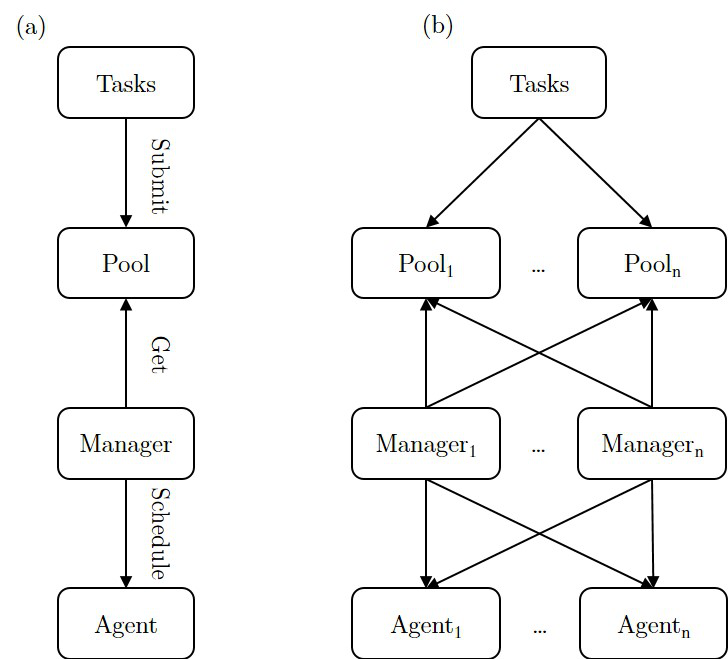
\includegraphics[width=0.45\textwidth]{figures/pilot_section3_1}
	\caption{(a) Components and transitions of a generalized pilot
		system; (b) Pilot systems may be composed of multiple
	  instances of the same components. \aznote{Bottom of figure
        is slightly cut off}}
	\label{fig:s3_pilot_diagram}
\end{figure}

\mtnote{Different pool implementations, ways to make tasks available to the manager: potential topics to discuss in Section 4?}

Functionally, a pilot is a system that allows for a user to gain exclusive - i.e. not shared - control over the scheduling and execution of her tasks. As shown in Figure~\ref{fig:s3_pilot_diagram}, users submit tasks to a `pool', a store where tasks are collected and made available to a manager. The implementation of a pool varies among \pilotjobs with the pool being a stand-alone component or a subsystem of a master, and storing only the state of tasks or having also a dedicated set of capabilities.

\mtnote{Vocabulary: manager}
\mtnote{Capabilities across different manager implementations: potential topic to discuss in Section 4?}

Within a pilot system, a manager is responsible for getting tasks from one or more pools and scheduling them into possibly multiple agents (Figure~\ref{fig:s3_pilot_diagram}). Managers can offer a vast array of capabilities and they greatly differ among \pilotjob implementations. Scheduling algorithms but also mechanisms to allocate dynamically resources to each task depending on availability and performance evaluations are typical examples of capabilities already offered, or potentially implementable, in this type of managers.

\mtnote{Vocabulary: agent}

Agents executes the tasks pushed by or pulled from one or more managers (Figure~\ref{fig:s3_pilot_diagram}). Clearly, an agent must have the right amount and type of resources for an appropriate extent of time in order to execute its tasks. As such, this requirement brings together pilots and jobs.

\mtnote{Vocabulary: Pilot Job}

A \pilotjob is a system that combines the conceptual constituents defined for both `pilot' and `job' but also add the distinctive concepts of `placeholder', `early binding' and `late binding' and `multi-level scheduling'. \jhanote{we should consider a diagram to help distinguish late and early binding}

\mtnote{Vocabulary: Placeholder}

In order to get resources, each agent - or group of agents - of a pilot system is scheduled by a user as a job within a given infrastructure. These jobs are eventually granted the requested amount of resources for the indicated period of time and their agents are executed. At this point, an agent becomes a placeholder for the set of resources that have been specified by and assigned to its job.

\mtnote{How different \pilotjob implementations deal with the peculiarities of the job submission system of different infrastructures; whether \pilotjobs implementations offer job-submission interoperability among different infrastructures: potential topics to discuss in Section 4?}

The submission process of agents depends on the capabilities exposed by the submission system of the targeted infrastructure. For example, users may or may not explicitly indicate a destination for where these jobs need to be scheduled, may have to use dedicated queues and may have to deal with limitations on what processes can be executed on a specific infrastructure. Particularly important in this context are networking capabilities as, without connectivity, agents would not be able to communicate with their managers and, ultimately, with the end users.

Once one or more placeholders become available on the given infrastructures, users can start to use a \pilotjob system to execute their tasks. Users own the placeholders and can run their tasks by means of the corresponding agents without having to deal with the job submission system of the infrastructure. 

\mtnote{Vocabulary: multi-level scheduling}
\mtnote{Different ways to implement task scheduling: potential topics to discuss in Section 4?}

Tasks are scheduled on the available placeholders by means of a dedicated scheduler, the pilot master or directly by the users depending on the \pilotjobs implementations. As two level of scheduling are involved - the one used to schedule the placeholders and the other used to schedule tasks on the placeholder - \pilotjobs are said to implement `multi-level scheduling' [ref] by means of scheduling overlay [cit].

\mtnote{Vocabulary: binding}
\mtnote{Binding capabilities; execution model: potential topics to discuss in Section 4?}

The act of assigning resources to tasks is called `binding'. Users partition the resources managed by means of a placeholder, including its time allocation, so to execute multiple tasks in parallel or sequentially. As the tasks require less time to complete than the total walltime assigned to the placeholder, users never incur in the overheads imposed by the job submission system of a given infrastructure. The resources of multiple placeholders may also be used at the same time so to achieve elaborated execution patterns. As usual, the flexibility of a \pilotjob execution model depends on the details of its implementation.

\mtnote{Vocabulary: early/late binding}
\mtnote{Late-binding capabilities: potential topics to discuss in Section 4?}

The control exercised by the users on their placeholders depends on the amount of information they include when submitting their tasks to a pool. Users may fully specify how and where a task should be executed or may leave the manager and agents to evaluate those parameters for them. The former is called `early binding' as users decide in advance how and where to execute their tasks, the latter is called `late binding' because, at submission time, how and where a task will be executed is unspecified.

Late binding requires specific capabilities. Manager(s) and agent(s) must be able to evaluate the requirements of the submitted tasks and maximize the efficiency of their binding depending on the peculiar properties, configuration and state of the resources made available through the placeholder(s). As such, in a late binding scenario, managers and agents may decide the amount of placeholders to use, the granularity of their partitions, the amount and type of the resources to allocate to the tasks and where such tasks should be executed. In an ideal late binding situation, users would be free only to specify high-level, resource-independent parameters for their tasks as, for example, the amount of time or money that should be spent for their execution.

\subsection{Different components of the Landscape}

\mtnote{The idea is to focus this subsection on the relationship between \pilotjob and the environment - re infrastructure - where its agents are scheduled and executed. The analysis should focus on the set of capabilities that pertain exclusively - at least in theory - to each domain. This would outline functionally and qualitatively the `landscape' of \pilotjob and offer a base for the critical analysis of the \pilotjobs implementations in \S 4. The idea would be to show how implementations choose ad hoc solutions depending on the specific characteristic of their landscape, both in terms of compensating for their limitations or exploiting their peculiarities. }

\begin{itemize}

    \item Resource Types

        \begin{itemize}
            \item HTC Grids
            \item HPC Grids
            \item Virtualized Environments (Clouds)
            \item Hybrids, Cloud-bursting, etc.
        \end{itemize}

    \item Organizational Structures

        \begin{itemize}
            \item Virtual Organizations
            \item "The XSEDE Model"
        \end{itemize}

    \item Software and Services \mtnote{this subsection would focus specifically on this item}

        \begin{itemize}
            \item Single-site, local workload mgmt. systems (HPC schedulers)
            \item Single-site endpoint services (e.g., GRAM, CREAM)
            \item Multi-site workload mgmt. systems (meta-scheduler)
            \item File transfer services
            \item Metadata services
        \end{itemize}

    \item Access Mechanisms

        \begin{itemize}
    	    \item API 
            \item CMD Line tools
            \item Gateways (web)
        \end{itemize}

    \item Applications and Use-Cases

        \begin{itemize}
            \item X
        \end{itemize}

\end{itemize}

\jhanote{Something akin to Matteo's diagram}

%\begin{itemize}
%        \item PJ abstractions are not defined in a void;
%	\item use cases, scientific practice and distributed applications;
%        \item heterogeneous DIs: grid, cloud and hybrids;
%	\item jobs and services;
%        \item LoAs implied by the PJ abstractions;
%	\item diagram.
%\end{itemize}
%
\subsection{Common Terms and Definitions}

\alnote{What to do with the terms, such as many-task computing, meta computing, grid computing, etc.? It might make sense to couple the evolution of \pilots to the evolution of these infrastructure paradigms (hypes). Maybe in history section.}

\mtnote{I think subsection 3.0 addresses this comment. If we all agree on todays call, I will comment out the entire subsection.}

\alnote{Can we start of with the P* elements so that we have something?}
\begin{itemize}
    \item application
    \item workflow
    \item pilot framework
    \item manager
    \item pilot, agent, executor, butler process, placeholder
    \item scheduler
    \item job
    \item workload
    \item ensemble
    \item \computeunit
    \item platform
\end{itemize}

% \mtnote{Following AndreL suggestion. Work in progress, I am still trying to map this list into \S2 + P*. The final version of the diagram will be based on these lists.}
% \begin{itemize}
%     \item Common concepts
%         \begin{itemize}
%              \item Placeholder
%              \item $\langle$Late binding/placement$\rangle$
%              \item $\langle$Master/worker$\rangle$
%              \item Workload
%              \item Job
%              \item \computeunit
%         \end{itemize}
%     \item Distinctive concepts
%         \begin{itemize}
%              \item $\langle$High-level framework$\rangle$
%              \item Workflow
%              \item Scheduler
%              \item Ensemble?
%         \end{itemize}
% \end{itemize}

%The terminology used to describe the implementations of pilot-job reviewed in
%section 2 varies depending not only on the type of implementation considered --
%simple/core, pilot-based scheduling and higher-level application framework --
%but also on the application domain where they are deployed and leveraged.
%Nonetheless, some common concepts can be identified so that a common vocabulary
%can be developed. The goal is to leverage such a vocabulary to ...
%\mtnote{what exactly do we want to achieve with Section 4?}.

%'Late-binding' is one of the concepts that persist unchanged across all the
%pilot-job implementations. 
%\begin{itemize}
%        \item Late-binding: 
%\end{itemize}
%
%The very same nature of pilot-job is that of enabling a late-binding of
%resources to jobs. This is what allows for a pilot-job to offer 'load
%balancing', 'scheduling' and to some extent 'domain distribution'. Late-binding
%is also directly related to the possibility for a pilot-job system to fulfil
%the qualitative requirements related to the efficiency with which jobs are
%distributed, scheduled and executed by the user on one or more distributed
%infrastructure. \mtnote{shall we assume these definitions? I think so but I
%want to be sure.}

%% \newpage

%% \begin{table*}[t]
%%   \footnotesize{
%%  \up
%%  \centering
%%  %\begin{tabular}{|p{2.5cm}|p{3cm}|p{3cm}|p{3cm}|p{3cm}|p{3cm}|p{3cm}|}
%%  \begin{tabular}{|p{2cm}|p{2cm}|p{2cm}|p{2cm}|p{2cm}|p{2cm}|p{2cm}|}
%%   \hline
%%   \textbf{Pilot Element}
%%   &\textbf{BigJob} &\textbf{DIANE} &\textbf{Condor-G/Glide-in} &\textbf{Swift/Coaster} &\textbf{Bosco} &\textbf{GWPilot}\\
%%   \hline
%%   Pilot-Manager &BigJob Manager & RunMaster & condor\_master, condor\_collector, condor\_negotiator, condor\_schedd &Coaster Service & Condor & Gridway\aznote{fill in}\\ 
%%   \hline
%%   \pilot &BigJob Agent  & Worker Agent &condor\_master, condor\_startd &Coaster Worker & condor\_master, condor\_startd& GWpilot\aznote{(?) check} \\
%%   \hline
%%   \computeunit  \ (CU) &Task &Task &Job &Application Interface Function (Swift Script) & Job & Task\\
%%   \hline
%%   \su \ (SU) &Sub-Job &Task &Job &Job & Job & Task \\
%%   \hline
%%   Data support & BigData& & & & &\\
%%   \hline
%%   Deployment (centrally hosted vs application)  & Application & & & &Runs locally, requires remote cluster install & Centrally hosted \aznote{Req. gridway install}\\
%%   \hline
%%   Interoperable & via SAGA & & & &Yes, via Condor & Yes, via BLAHPD\\
%%   \hline
%%   Abstraction(?) & & & & & &\\
%%   \hline
%%   Coordination(?) &Advert & & & & &\\

%% % \hline
%% % Dynamic Resources &no/yes &yes (AgentFactories)\\
%%  \hline
%%  \end{tabular}
%%  \caption{\textbf{Comparing PJ Systems} 
%%    Exposing the commonalities of PJ systems \aznote{Some of these are going to be almost identical e.g. Bosco w/
%%      Condor -- combine their columns to emphasize similarity?} \aznote{properly formatted later once complete/judged relevant}
%%    \aznote{Not sure of relevance of an ``all-encompassing table'' if we are
%%      going to be focusing on ``landmark'' Pilot-Job systems...
%%      put this on the back-burner for the time being..}
%%  \up
%%  } 
%%  \label{table:bigjob-saga-diane}
%% }
%% \end{table*}


%% \begin{landscape}
%% \begin{table}
%% \begin{center}
%% \begin{footnotesize}
%% \begin{tabular}{|p{3.0cm}|p{3.5cm}|p{2.3cm}|p{1.9cm}|p{3.7cm}|p{2.5cm}|}
%% \hline {\bf BigJob}
%% & {\bf Diane}
%% & {\bf Condor/Glide-in}
%% & {\bf Swift}
%% & {\bf Bosco}
%% & {\bf GWPilot}
%% \\
%% \hline

%% Montage
%% & Multiple sequential and parallel executables
%% & Files
%% & Dataflow (DAG)
%% & Dynamic process creation, workflow execution, file transfer
%% & test
%% \\
%% \hline

%% \end{tabular}
%% \end{footnotesize}
%% \caption{\label{Tab:AppChars} }
%% \end{center}
%% \end{table}
%% \end{landscape}

\section{Pilot-Job Systems Revisited}
\aznote{Ashley's section}
Despite the apparent diversity in existing Pilot-Jobs,
they can be reduced to a set of common functionality and
discussed as such.  This reduction has implications
for the interoperability of existing and future Pilot-Jobs, and
lends insight into application design to enhance job/data(?)
mobility, management, and potential run-time responsiveness via
late-binding/etc.  We will see that throughout the evolution
of the Pilot-Job concept, several core concepts have remained stable
while new additions enhance cross-platform interoperability,
ease of usage and deployment, and add the ability to
schedule data as well as jobs. \aznote{Check this
sentence later to make sure it is not overreaching}


\jhanote{Ashley to ``finish'': AppLeS, MyCluster and PANDA: Ole to
  finish Glide-in, Corral and Bosco: Mark to finish DIANE,
  Swift/falkon, DIRAC(?)}


\subsection{Comparing Pilot-Jobs via a Common Framework \& Vocabulary}
\aznote{Ashley's section}

In light of the common vocabulary discussion in 
Section~\ref{sec:vocab}, a representative set of Pilot-Jobs
has been chosen for further analysis.  

\aznote{Two approaches here:  this is the first}

Each Pilot-Job is from a respective categorization from
Section~\ref{sec:survey}.  Examining each of these Pilot-Jobs via a
common vocabulary exposes their core similarities, and allows a
detailed analysis of their differences.

\aznote{And the second potential approach}
Representative Pilot-Jobs from each Pilot-Job category
in Section~\ref{sec:survey} are chosen and compared within
the bounds of that category, illustrating the core similarities
between the Pilot-Jobs in a given category.

\aznote{Either approach requires the best ``representative PJs''
  to be chosen.  This is more important if we pick just one of
  each, of course...}

Finally, we perform
a cross-cutting analysis, demonstrating that across the categorical
distinctions all approaches remain true ``Pilot-Jobs'' with regard
to their base functionality.  The segmentation between categories
is exposed to reveal why Pilot-Jobs have evolved to have
differing capabilities, with the end-goal being a
complete understanding of the Pilot-Job ecosystem via a common
vocabulary.

%\subsubsection{Condor-G}
%% \aznote{Section copied and pasted from IPDPS paper for now -- plan
%% to use this general sort of information + reword using our spiffy 
%% vocabulary presented in this paper}
%% Condor-G pioneered the Pilot-Job concept~\cite{condor-g}. The pilot is
%% actually a complete Condor pool that is started using the Globus
%% service of a resource. This mechanism is referred to as Condor
%% Glide-In. Subsequently, jobs can be submitted to this Glide-In pool
%% using the standard Condor tools and APIs. Condor utilizes a
%% master/worker coordination model. The PJ manager is referred to as the
%% Condor Central Manager. The functionality of the Central Manager is
%% provided by several daemons: the condor\_master that is generally
%% responsible for managing all daemons on a machine, the
%% condor\_collector which collects resource information, the
%% condor\_negotiator that does the matchmaking and the condor\_schedd
%% that is responsible for managing the binding and scheduling
%% process. Condor generally does not differentiate between workload,
%% i.\,e.\ WU, and schedulable entity, i.\,e.\ SU. Both entities are
%% referred to as job. However, it supports late binding, i.\,e.\
%% resources a job is submitted to must generally not be available at
%% submission time. The scheduler matches the capabilities required by a
%% WU to the available resources. This process is referred to as
%% matchmaking. Further, a priority-based scheduler is used. For
%% communication between the identified elements Condor utilizes
%% point-to-point messaging using a binary protocol on top of TCP.

%% Different fault tolerance mechanisms, such as automatic retries, are
%% supported.  Further, Condor supports different security mechanisms:
%% for authentication it integrates both with local account management
%% systems (such as Kerberos) as well as grid authentication systems such
%% as GIS. Communication traffic can be encrypted.
\subsubsection{AppLeS - Pre-PJ-Systems / Master/Worker frameworks}
\aznote{Resource discovery a special feature, as well as performance-modelling
for resource selection}
Scheduling/resource-selection is handled by a per-application AppleS agent.
Although many features from more advanced pilot systems are missing, a subset
of \pilotjob functionality such as late-binding and 
application-level scheduling are present in AppLeS.
However, the lack of a placeholder job limits the functionality 
of late-binding and application-level scheduling, as tasks
must wait in unpredictable queues before being executed,
undermining the level of contol.

\aznote{\url{http://www.sc2000.org/techpapr/papers/pap.pap169.pdf} - Also consider this paper:
The AppLeS Parameter Sweep Template: User-Level Middleware for the Grid?}

\aznote{Talk about how what AppLeS is missing to be a true PJ system}

\subsubsection{MyCluster - Basic Pilot-Job Systems}
MyCluster~\cite{1652061}...
\aznote{Didn't pick Condor-G/Glide-in, as GlideinWMS uses Condor as well and did not
want to have two Condor-based pilots...  but maybe that would make things look nicer
and show a natural evolution?}
\begin{itemize}
\item Master Node Manager = Manager \aznote{Master Node
Manager process within a GNU Screen session that then
starts the Condor/SGE master daemons in user space if
needed.}
\item Agent Manager \aznote{ The
agent manager remotely executes a Proxy Manager process at
each participating site using Globus GRAM}
\item Submission Agent
\item Proxy Manager
\item Task Manager = pilot
\item Slave-node managers = compute units (?) 
  \aznote{The slave node managers are responsible for starting the
    Condor or SGE job-starter daemons. These daemons connect
    back to the master processes on the client workstation, or to a
    pre-existing departmental cluster, depending on the virtual
    login configuration.
  }
\item Job proxy (?)
\end{itemize}


\subsubsection{GlideinWMS - Pilot-based Scheduling/Multi-Level Scheduling}
\textit{Collectors} are the managers, with one collector per
GlideinWMS system.
\textit{Glidein factory daemon}s are responsible for
submitting pilot jobs to grid pools\aznote{Use diff vocab for grid pool?}.
They therefore correspond to pilot managers.
\textit{VO frontend daemons} are the schedulers, which map jobs
to pilots.  GlideinWMS takes advantage of late-binding, as
jobs are not selected for resources until the pilots start.\aznote{This
should be true of all systems described in this section -- do we
need to explicitly say so for each pilot system?}
\textit{WMS collector machine} manages communication between the glidein
factory daemons(pilot managers) and VO frontend daemons(schedulers)
and so corresponds to \aznote{We don't have anything for this.  This
sounds like what REDIS/etc do for BJ though.  Should we incorporate this
into our vocabulary?}
\textit{User jobs} correspond to compute units \aznote{Right?}

\begin{itemize}
%Unlisted things \\
\item Workflow (doesn't seem to be explicit support)
\item Workload (is this just a list of user jobs that are queued up)
\item Placeholder (isn't this the same kind of deal as a Pilot-Job/PJ
waiting in a queue?)
\item Pilot framework (The entire GlideinWMS qualifies as a ``pilot
framework'', correct?)
\item Ensemble \aznote{How to tie this in}
\item Platform \aznote{Ditto}
\item Master-Worker \aznote{Likewise, we could say that the
VO factory daemons are the masters with the pilots the workers,
but this seems overly pedantic?}
\end{itemize}

\subsubsection{Corral - 2nd Pilot-based Scheduling/Multi-Level Scheduling}
\aznote{SJ asked for an investigation of Corral -- not sure that this
deserves a full analysis at this point on a technical level despite
being commonly used, open to suggestions}

Corral is designed to allow hybrid HTC/HPC execution, in which
many small jobs may be executed in conjunction with larger runs. 
\cite{Rynge:2011:EUG:2116259.2116599}
\aznote{Back this up w/ paper refs -- paper is somewhat dated,
verify this is still true today}.  Corral operates as a Glidein
WMS frontend\aznote{main reason that I think we shouldn't include
Corral in its own section...}, where GlideinWMS manages the size
of Condor glide-in pools.
\begin{itemize}
\item Workflow - handled by Pegasus workflow management system
  \aznote{True in the paper I am using, but not handled by Corral itself, so should we include this?}
\item Placeholder - handled by multislot requests 
  \aznote{multislot request requests a single large
    GRAM job, and then starts glideins within this container}
\item Job
\item Compute unit
\item Workload 
\item Will fill this in later...
\end{itemize}

\subsubsection{Swift - Higher-Level Application Frameworks (Workflow)}

\subsubsection{DIANE - Higher-Level Application Frameworks 
  (Task Farming/Master-Worker)}
\aznote{Do we want to define single-user vs multi-user? 
  Communication methods?  Output aggregrator?}

\aznote{DIANE runmaster/etc not included in current paper we
have cited}

DIANE~\cite{Moscicki:908910} is a task coordination framework, which
was originally designed for implementing master/worker applications,
but also provides PJ functionality for job-style executions.
DIANE utilizes a single hierarchy of worker agents as well as a PJ \textit{manager}
referred to as \texttt{RunMaster}.  The manager creates
placeholders called \texttt{Workers}, which register with and receive jobs from the manager.
%For the spawning of PJs a separate script, the so-called submitter script, is
%required. 
The \textit{scheduler} for DIANE is known as the \texttt{Planner}.
%For the access to the physical resources the GANGA
%framework~\cite{Moscicki20092303} can be used.
%A worker agent generally manages only a single
%core and thus, by default is not able to run parallel applications.
% Once the worker agents are started they register themselves at the RunMaster.
% GANGA provides a
% unified interface for job submissions to various resource types, e.\,g.\ EGI
% resources or TG resources via a SAGA backend.
%DIANE operates on the master-worker computing model.

%The \textit{manager} for DIANE is called the \texttt{Master}, and contains
%the \textit{scheduler} for DIANE, which is known as the \texttt{Planner}.
%The manager creates placeholders called \texttt{Workers}, which
%register with and receive jobs from the manager.

The workflow is then such that a user submits a parallel job to
the grid using a DIANE client.  The client then creates the Pilot manager
and remains in contact with it to control its \pilotjobs.  Results
are aggregated through use means of the DIANE
\texttt{Integrator}.\aznote{No mapping vocab for the integrator as of now.}
DIANE includes a simple capability matcher and FIFO-based task scheduler
to help facilitate the execution of jobs.
Plugins for other workloads, e.\,g.\ DAGs or for data-intensive
application, exist or are under development. The framework is extensible:
applications can implement a custom application-level scheduler.

For communication between the RunMaster and
worker agents point-to-point messaging based on CORBA~\cite{OMG-CORBA303:2004}
is used. CORBA is also used for file staging.
DIANE is a single-user PJ, i.\,e.\ each PJ is executed with the
privileges of the respective user. Also, only WUs of this respective user can be
executed by DIANE. DIANE supports various middleware security mechanisms
(e.\,g.\ GSI, X509 authentication). For this purpose it relies on GANGA. The
implementation of GSI on TCP-level is possible, but currently not yet
implemented. Further, DIANE supports fault tolerance: basic error detection and
propagation mechanisms are in place. Further, an automatic re-execution of WUs
is possible.

DIANE is primarily designed with respect to HTC environments (such as
EGI~\cite{egi}), i.\,e.\ one PJ consists of a single worker agent with the
size of 1 core.


\subsubsection{Bosco - Higher-Level Application Frameworks 
  (Data Analytics and Visualization)}

%% \aznote{Section copied and pasted from IPDPS paper for now -- plan
%% to use this general sort of information + reword using our spiffy 
%% vocabulary presented in this paper}
%% % Coordination and Communication
%% DIANE~\cite{Moscicki:908910} is a task coordination framework, which
%% was originally designed for implementing master/worker applications,
%% but also provides PJ functionality for job-style executions. DIANE
%% utilizes a single hierarchy of worker agents as well as a PJ manager
%% referred to as \texttt{RunMaster}.
%% %Further, there is ongoing work on a multi-master extension.
%% For the spawning of PJs a separate script, the so-called submitter script, is
%% required. For the access to the physical resources the GANGA
%% framework~\cite{Moscicki20092303} can be used.
%% %GANGA provides a
%% %unified interface for job submissions to various resource types, e.\,g.\ EGI
%% %resources or TG resources via a SAGA backend.
%% Once the worker agents are started they register themselves at the RunMaster.
%% In contrast to TROY-BigJob, a worker agent generally manages only a single
%% core and thus, by default is not able to run parallel applications (e.\,g.\
%% based on MPI). BJ utilizes the BJ-Agent that is able manage a set of local
%% resources (e.\,g.\ a certain number of nodes and cores) and thus, is capable
%% of running parallel applications. For communication between the RunMaster and
%% worker agents point-to-point messaging based on CORBA~\cite{OMG-CORBA303:2004}
%% is used. CORBA is also used for file staging, which is not fully supported by
%% BJ, yet.

%% % Binding 
%% DIANE is primarily designed with respect to HTC environments (such as
%% EGI~\cite{egi}), i.\,e.\ one PJ consists of a single worker agent with the
%% size of 1 core. BJ in contrast is designed for HPC systems such as TG,
%% where a job usually allocates multiple nodes and cores. To address this issue
%% a so-called multinode submitter script can be used: the scripts starts a
%% defined number of worker agents on a certain resource. However, WUs will be
%% constrained to the specific number of cores managed by a worker agent. A
%% flexible allocation of resource chunks as with BJ is not possible. By
%% default a WU is mapped to a SU; application can however implement smarter
%% allocation schemes, e.\,g.\ the clustering of multiple WUs into a SU.

%% %Scheduling
%% DIANE includes a simple capability matcher and FIFO-based task scheduler.
%% Plugins for other workloads, e.\,g.\ DAGs or for data-intensive
%% application, exist or are under development. The framework is extensible:
%% applications can implement a custom application-level scheduler.


%% %Other impl. related issues: FT and security
%% DIANE is, just like BJ, a single-user PJ, i.\,e.\ each PJ is executed with the
%% privileges of the respective user. Also, only WUs of this respective user can be
%% executed by DIANE. DIANE supports various middleware security mechanisms
%% (e.\,g.\ GSI, X509 authentication). For this purpose it relies on GANGA. The
%% implementation of GSI on TCP-level is possible, but currently not yet
%% implemented. Further, DIANE supports fault tolerance: basic error detection and
%% propagation mechanisms are in place. Further, an automatic re-execution of WUs
%% is possible.


%% \aznote{Section copied and pasted from IPDPS paper for now -- plan
%% to use this general sort of information + reword using our spiffy 
%% vocabulary presented in this paper}
%% Swift~\cite{Wilde2011} is a scripting language designed for expressing
%% abstract workflows and computations. The language provides, amongst many other
%% things, capabilities for executing external applications, as well as the
%% implicit management of data flows between application tasks. 
%% % For this
%% % purpose, Swift formalizes the way that applications can define
%% % data-dependencies. Using so called mappers, these dependencies can be
%% % easily extended to files or groups of files. 
%% The runtime environment handles the allocation of resources and the spawning of 
%% the compute tasks. 
%% % Both data- and execution management capabilities are provided
%% % via abstract interfaces. 
%% Swift supports e.\,g.\ Globus, Condor and PBS resources. 
%% % The pool of resources
%% % that is used for an application is statically defined in a configuration file.
%% % While this configuration file can refer to highly dynamic resources (such as OSG
%% % resources), there is no possibility to manage this resource pool
%% % programmatically. 
%% By default, Swift uses a 1:1 mapping for \cus and \sus. However,
%% Swift supports the grouping of SUs as well as PJs. For the PJ functionality, Swift uses the
%% Coaster~\cite{coasters} framework. Coaster relies on a master/worker
%% coordination model; communication is implemented using GSI-secured TCP sockets.
%% Swift and Coaster support various scheduling mechanisms, e.\,g.\ a FIFO and a
%% load-aware scheduler. Additionally, Swift can be used in conjunction with 
%% Falkon~\cite{1362680}, which also provides \pilot-like functionality.

%% % Falkon
%% % refers to \pilots as the so called provisioner, which are created using the
%% % Globus GRAM service. The provisioner spawns a set of executor processes on the
%% % allocated resources, which are then responsible for managing the execution of
%% % SUs. \cus are submitted via a so called dispatcher service. Similar to Coaster,
%% % Falkon utilizes a M/W coordination model, i.\,e.\ the executors periodically
%% % query the dispatcher for new SUs. Web services are used for communication.

%\subsubsection{GWPilot}
%% \aznote{Considering the new direction of the paper, I am not sure whether
%% GWPilot~\cite{gwpilot} requires its own section for analysis...}

%% %\begin{lstlisting}[breaklines]
%% %\url{https://indico.egi.eu/indico/materialDisplay.py?contribId=18&sessionId=46&materialId=slides&confId=1019}
%% %\url{http://ieeexplore.ieee.org/xpls/abs_all.jsp?arnumber=6266981}
%% \begin{itemize}
%% \item Integrates with GridWay metascheduler
%% \item Pilots advertise to GridWay, GridWay scheduler schedules pilots
%% \item Pilots pull tasks from scheduler
%% \item Installation as a GridWay driver -- written in Python
%% \item Interoperability managed by GridWay drivers (DRMAA, JDSL, BES, more?)
%% \item Using GWPilot requires only adding a single line to their GridWay task
%% \item ``Lightweight and scalable''
%% \end{itemize}
%% %\end{lstlisting}

%\subsubsection{Bosco}
%% \aznote{Given the modified direction we are taking the paper (``landmark''
%% pilot-jobs reviewed as opposed to all-inclusive), I suggest nixing
%% the inclusion of Bosco~\cite{bosco} in this section as Bosco appears
%% to be mostly making strides with regards to user-accessibility
%% of pilots.}
%% \\
%% \begin{itemize}
%% \item Condor used as batch system/user interface
%% \item Single submit model for different cluster types (LSF/PBS/SGE/etc) via SSH with \texttt{BLAHPD}
%% \item Campus Factory (condor overlay generator) creates glideins, checks users queue for idle jobs, 
%%   enforces submission policies
%% \item Bosco = ``BLAHPD Over SSH Condor Overlay''
%% \item Workstation-based (run Bosco client locally)
%% \item Multi-user (Bosco workstation install can be used by multiple researchers)
%% \item Supports multiple cluster submission (but what about coordination...)

%% \end{itemize}
% \upp
% \subsection{SWIFT-Coaster\upp\upp}
% 
% SWIFT~\cite{Wilde2011} is a scripting language designed for expressing abstract
% rest of this cut, but making a note of this in case we want
% to bring swift into the discussion later that i can find more info in 2011 paper
%\aznote{Much of what I was thinking of doing is similar to the 2011 IPDPS paper
%in the 2012-PStar directory.  Is this along the right lines?}

%\aznote{A bit confused about how to tie this into conclusion and discussion:
%``The need for a common minimum model'' in particular.  I am guessing that
%I should help to ``set up'' that section by providing plenty of material showing
%that the pilot job systems are very similar at their core.  How far should I
%go with this, however, to avoid hitting the ``conclusion'' material in this section?
%}



\section{Conclusion and Discussion}

\jhanote{Main message is: (i) \pilotjobs have potential, but it is not
  being realized due to ad hoc nature of theory and practise, (ii) we
  provide first comprehensive historical and technical analysis, (iii)
  set the stage for a common conceptual model and implementation
  framework, and (iv) provide insight and lessons for other tools and
  higher-level frameworks, such as Workflow systems possibly}


\subsection{The need for a common minimum model}

%Whereas we will discuss in greater detail some of the concepts upon
%which this paper is built, for completeness we briefly outline them
%here.

Our initial investigation~\cite{Luckow:2008la} into
\pilot-Abstractions was motivated by the desire to provide a single
conceptual framework --- referred to as the P* Model, that would be
used to understand and reason the plethora and myriad \pilotjob
implementations that exist.

 
Once a common and uniform conceptual model was available, the notion
of \pilotdata was conceived using the power of symmetry, i.e., the
notion of \pilotdata was as fundamental to dynamic data placement and
scheduling as \pilotjobs was to computational tasks. As a measure of
validity, the \pstar model was amenable and easily extensible to
\pilotdata.  The consistent and symmetrical treatment of data and
compute in the model led to the generalization of the model as the
{\it P* Model of Pilot Abstractions}.


\subsection{Lessons for Workflow System}

The current state of workflow (WF) systems~\cite{nsf-workflow,1196459}
provides a motivating example for the P* Model and the Pilot-API: even
though many WF systems exist (with significant duplicated effort),
they provide limited means for extensibility and interoperability.  We
are not naive enough to suggest a single reason, but assert that one
important contributing fact is the lack of the right interface
abstractions upon which to construct workflow systems; had those been
available, many/most WF engines would have likely utilized them (or
parts thereof), instead of proprietary solutions.

% That would not immediately allow WF implementations to interoperate,
% but would make semantic mapping between them significantly simpler,
% thus supporting the very notion of interoperation.

Significant effort has been invested towards WF interoperability at
different levels -- if nothing else, providing post-facto
justification of its importance. The impact of missing interface
abstractions on the WF world can be seen through the consequences of
their absence: WF interoperability remains difficult if not
infeasible. The Pilot-API in conjunction with the P* Model aims to
prevent similar situation for \pilotjobs.

\note{What is the future of PJ? Why should we do to enhance the usability?}

%\footnote{To be fair: we are not sure if a generic model and/or a
%  generic WF API are achievable {\it on a useful level} -- we think,
%  nevertherless, that our discussion is valid.}



%\mrnote{We have a survey of related \pilotjobs systems, a 'history'
%of \pilotjobs, and a related work section? Not sure if we should
%condense in some way. PS Why is this after conclusion?}

%\subsection{Scientific Data Management}


\section*{Acknowledgements}
{\footnotesize{This work is funded by NSF CHE-1125332 (Cyber-enabled
  Discovery and Innovation), NSF-ExTENCI (OCI-1007115) and
  ``Collaborative Research: Standards-Based Cyberinfrastructure for
  Hydrometeorologic Modeling: US-European Research Partnership''
  (OCI-1235085) and Department of Energy Award (ASCR)
  DE-FG02-12ER26115.  This work has also been made possible thanks to
  computer resources provided by TeraGrid TRAC award TG-MCB090174 and
  BiG Grid.  This document was developed with support from the US NSF
  under Grant No. 0910812 to Indiana University for ``FutureGrid: An
  Experimental, High-Performance Grid Test-bed''.}}

% \bibliographystyle{IEEEtran}
\bibliographystyle{abbrv}
\bibliography{pilotjob,literatur,saga,saga-related}


\end{document}

